% id: 86-28
% book: 베이직쎈 미적분1 · 05 도함수의 활용 (2)
% section: 개념 39 함수의 최대와 최소의 활용
% figure: tikz:fig-86-28
% answer: 
% answer_source: 
% variant_level: 0 (원본 전사)
% 이 파일은 build.mjs 가 items.json 에서 만든다. 고칠 때는 items.json 을 고친다.
\smash{\raisebox{1.5mm}{\dmkichul{베이직쎈 미적분1 86쪽 28번}}}
\noindent\begin{minipage}[t]{0.58\linewidth}\vspace{0pt}\raggedright 오른쪽 그림과 같이 한 변의 길이가 12인 정사각형 모양의 종이의 네 귀퉁이에서 같은 크기의 정사각형을 잘라 내고 나머지 부분을 접어서 뚜껑이 없는 직육면체 모양의 상자를 만들려고 한다. 잘라 내는 정사각형의 한 변의 길이를 $x$라 할 때, 다음에 답하시오.\end{minipage}\hfill\begin{minipage}[t]{0.4\linewidth}\vspace{0pt}\centering \resizebox{\ifdim\width>\linewidth\linewidth\else\width\fi}{!}{% 86-28(86쪽) — 한 변의 길이가 12인 정사각형 종이의 네 귀퉁이에서 같은 크기의 정사각형을 잘라 낸 전개도. 스캔 화질이 낮아 TikZ 로 다시 그림.
% 원문에 있는 것만: 회색으로 칠한 남은 부분 · 잘라 낸 네 귀퉁이(흰 정사각형) · 접는 선(점선) · 치수 12 둘(점선 호). 잘라 내는 정사각형의 한 변 x 는 원문에 값이 없으므로 적지 않는다.
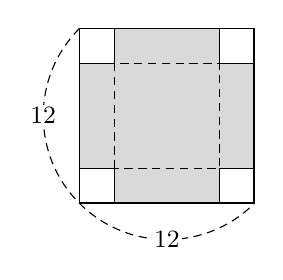
\begin{tikzpicture}[x=0.185cm, y=0.185cm, line width=0.5pt]
  \fill[black!15] (0,0) rectangle (12,12);
  \fill[white] (0,9.6) rectangle (2.4,12);
  \fill[white] (9.6,9.6) rectangle (12,12);
  \fill[white] (0,0) rectangle (2.4,2.4);
  \fill[white] (9.6,0) rectangle (12,2.4);
  \draw[line width=0.6pt] (0,0) rectangle (12,12);
  \draw[line width=0.6pt] (2.4,12) -- (2.4,9.6) -- (0,9.6);
  \draw[line width=0.6pt] (9.6,12) -- (9.6,9.6) -- (12,9.6);
  \draw[line width=0.6pt] (2.4,0) -- (2.4,2.4) -- (0,2.4);
  \draw[line width=0.6pt] (9.6,0) -- (9.6,2.4) -- (12,2.4);
  \draw[densely dashed, line width=0.4pt] (2.4,2.4) rectangle (9.6,9.6);
  \draw[densely dashed, line width=0.4pt] ([shift=(135:8.49)]6,6) arc (135:315:8.49);
  \node[fill=white, inner sep=1pt, font=\small] at (-2.49,6) {$12$};
  \node[fill=white, inner sep=1pt, font=\small] at (6,-2.49) {$12$};
\end{tikzpicture}
}\end{minipage}\par
\dmsubprob{1} 상자의 밑면의 한 변의 길이를 $x$에 대한 식으로 나타내시오.
\dmsubprob{2} $x$의 값의 범위를 구하시오.
\dmsubprob{3} 상자의 부피를 $V(x)$라 할 때, $V(x)$를 구하시오.
\dmsubprob{4} 상자의 부피의 최댓값을 구하시오.
